%-----------------------------------------------------------------------------------------------------
\chapter{Introduction}
%-----------------------------------------------------------------------------------------------------

%-----------------------------------------------------------------------------------------------------
\section{Work Description}
%-----------------------------------------------------------------------------------------------------

Over the past few decades, the fast development of wireless communication technologies has reinforced the importance of antennas as fundamental components of transmission and reception systems. A key parameter in antenna characterisation is the radiation pattern, which reveals how electromagnetic energy is distributed in space. Understanding and measuring this pattern is essential for evaluating antenna performance, optimising coverage, and ensuring efficient energy transfer. 

Existing commercial setups offer high accuracy, but are financially impractical for educational laboratories. For undergraduate environments, where the primary objective is to support teaching and provide hands-on experience, the investment in such equipment is frequently unjustifiable. In this context, the development of low-cost and custom-made solutions becomes relevant, enabling students to gain practical insights into antenna behaviour without requiring highly specialised or costly instrumentation.

This project addresses this need by developing a two-axis mechatronic and computerised system for antenna radiation pattern measurement. The system operates in the ISM band (below 1~GHz), specifically around 868 MHz, and combines mechanical design, custom electronics, and software integration. It includes stepper motors for antenna positioning, an Arduino-based control platform, a Radio Frequency (RF) power detector, and MATLAB\footnote{A campus version of this software is licensed to the Polytechnic Institute of Bragança.} for data acquisition and visualisation. An overview of the complete system is illustrated in Figure \ref{cap1:sec1:fig1}. To ensure signal integrity and accurate power transfer, the setup also incorporates an impedance matching network and a balun for common-mode current suppression. The system was validated by comparing experimental results with simulations of a Yagi–Uda antenna, serving as a proof of concept for its applicability in laboratory environments.

\begin{figure}[H]
\centering
\begin{subfigure}{0.25\textwidth}
\centering
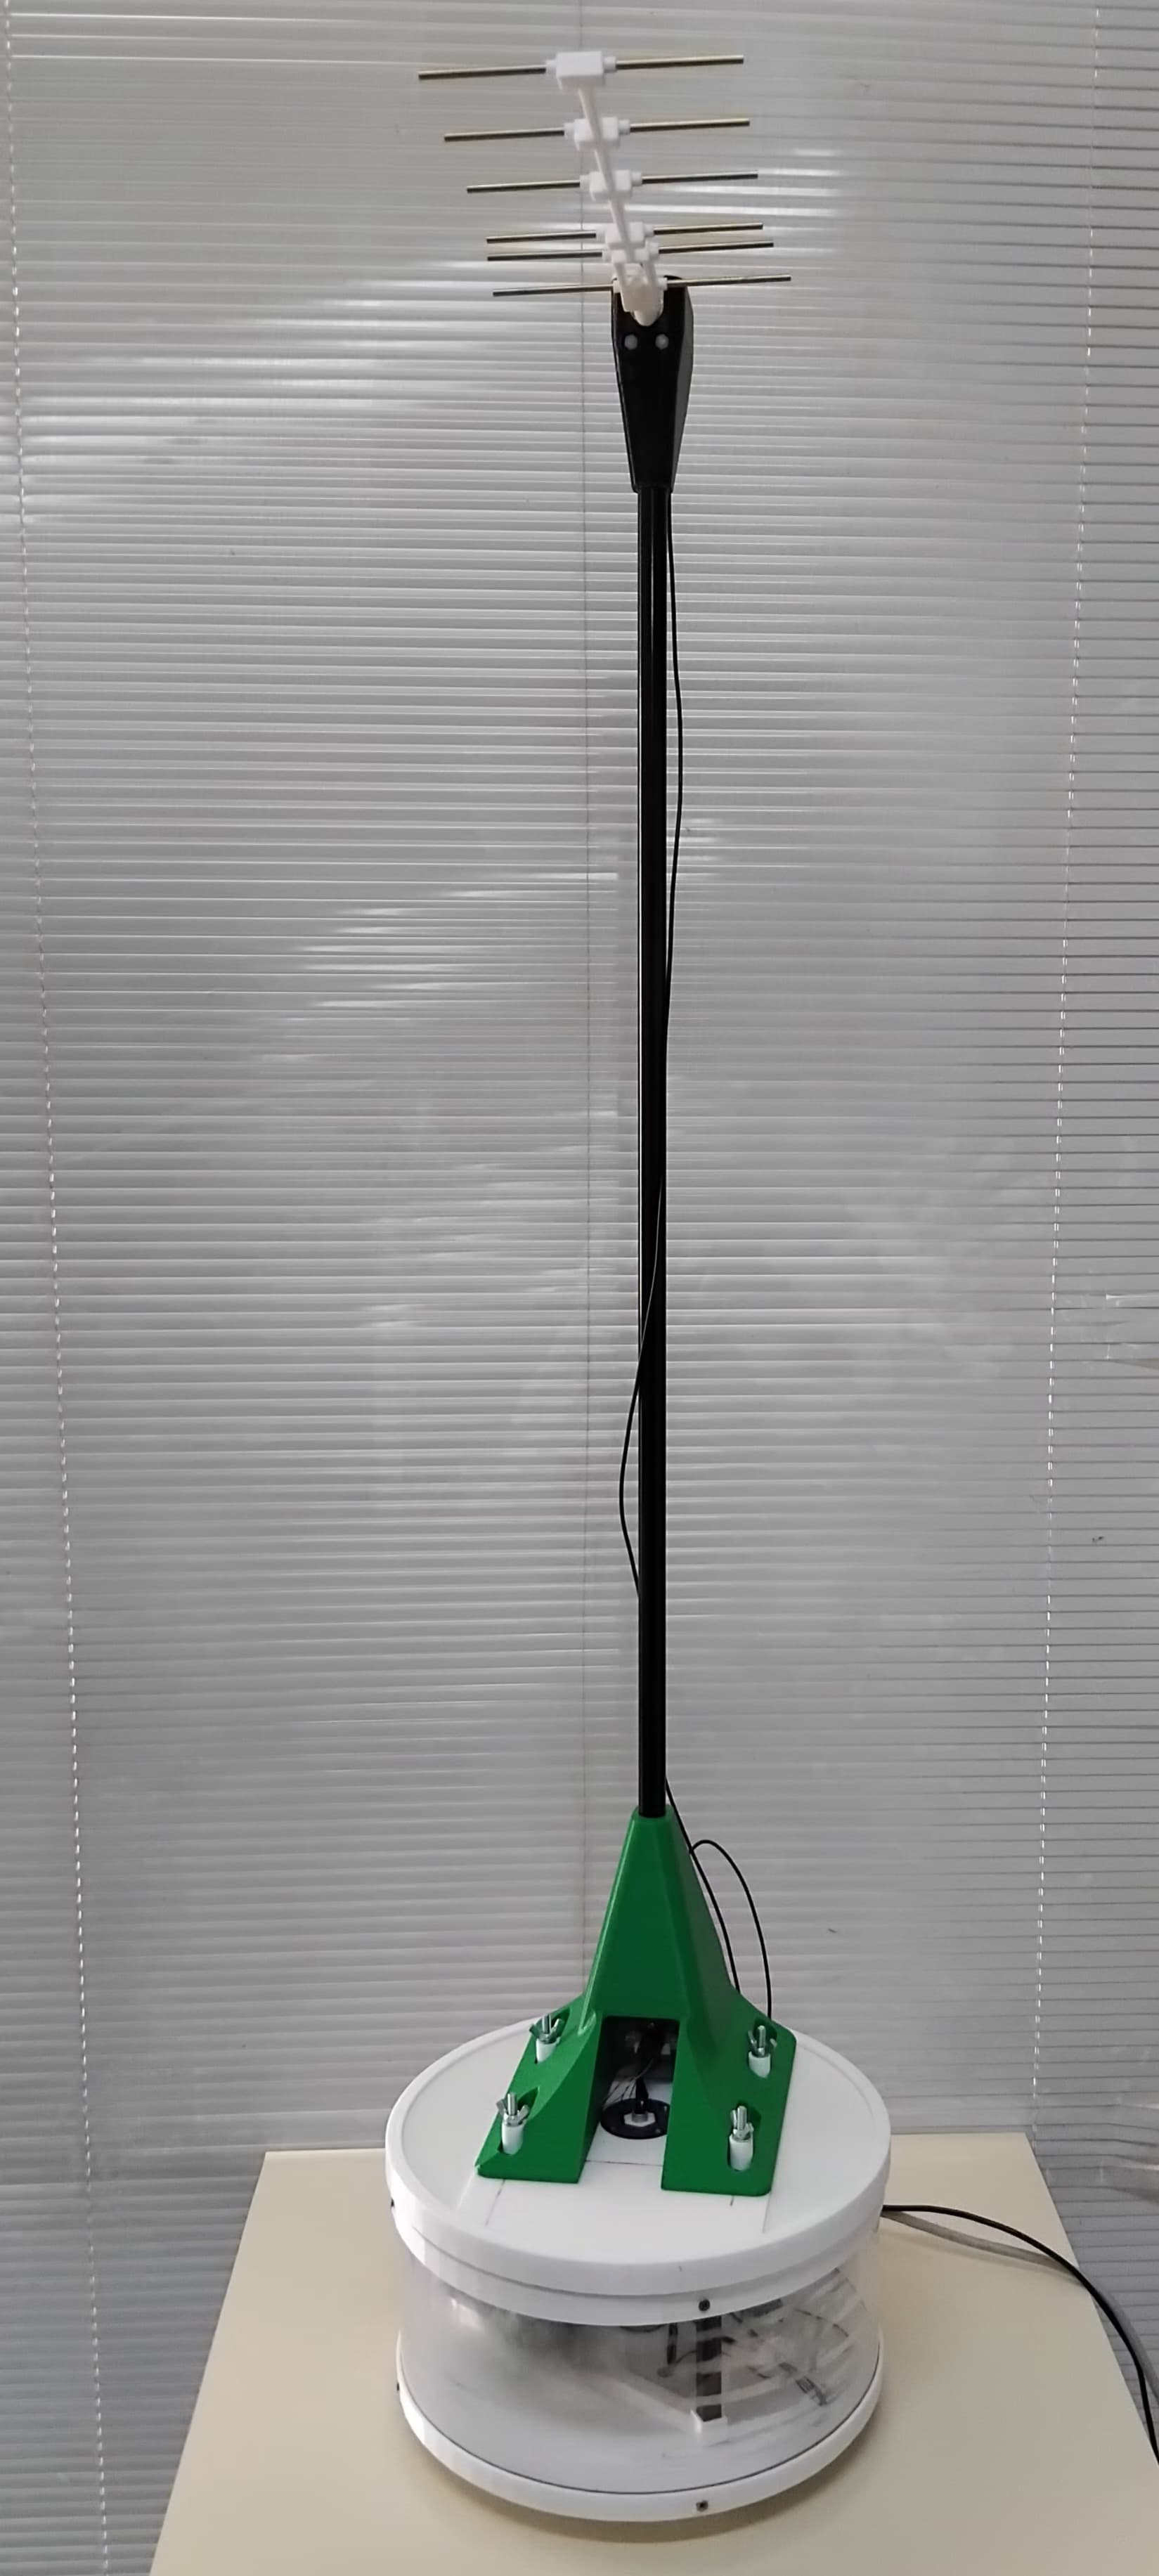
\includegraphics[width=\textwidth]{Imagens/front_view.jpg}
\caption{Front view}
\label{cap1:sec1:fig1:a}
\end{subfigure}
\hspace{3mm}
\begin{subfigure}{0.2555\textwidth}
\centering
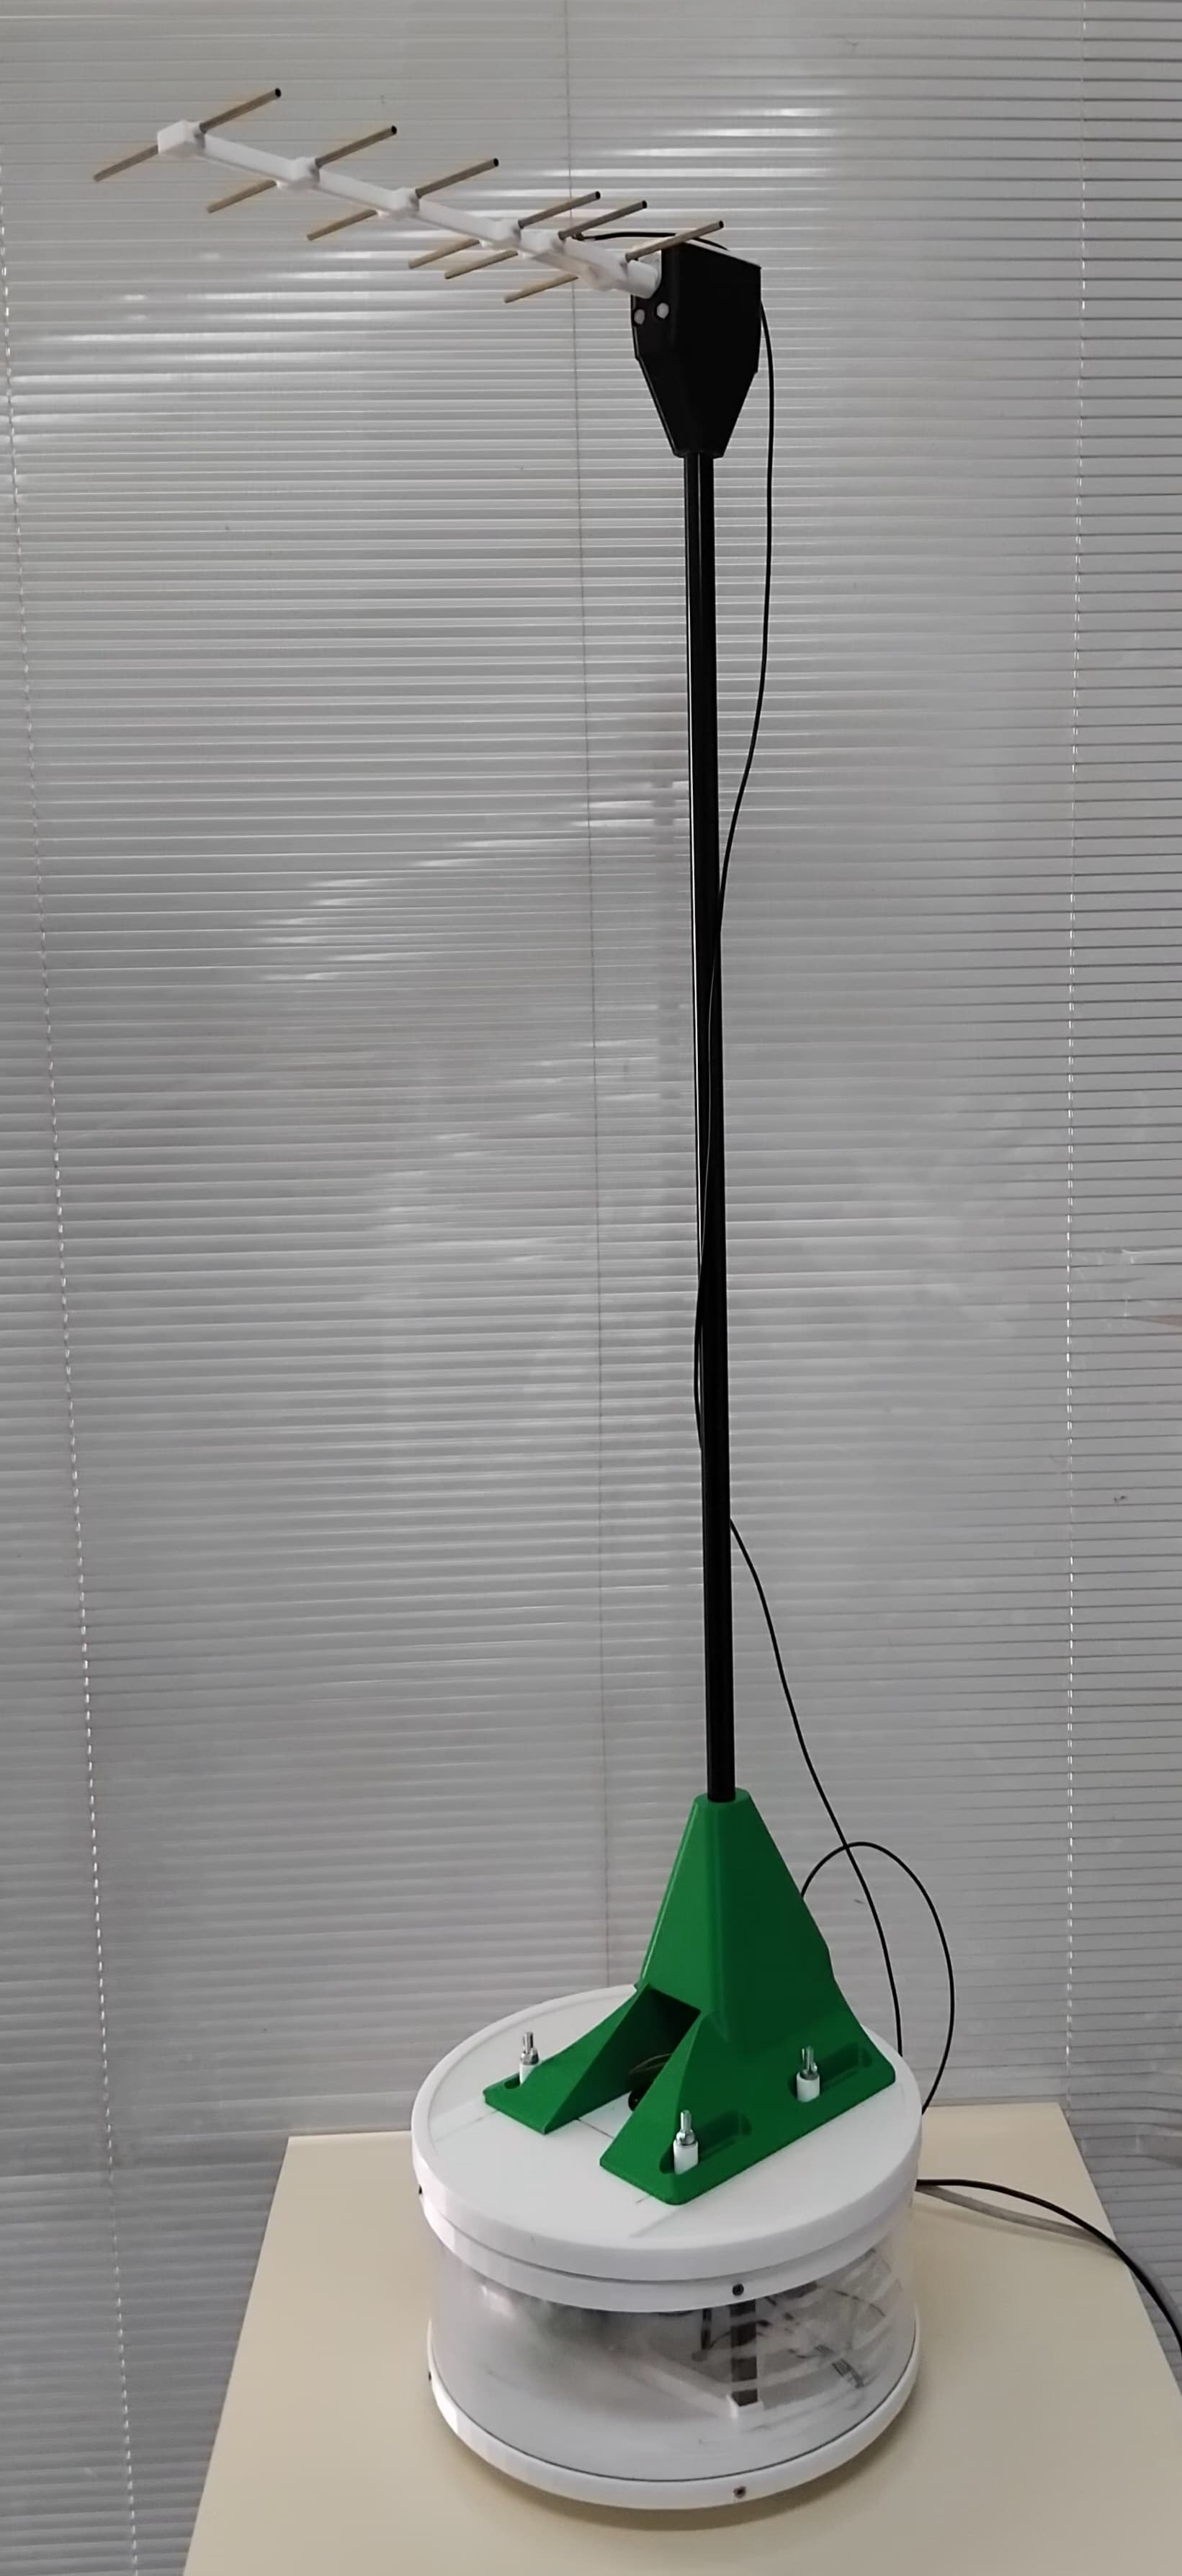
\includegraphics[width=\textwidth]{Imagens/side_view.jpg}
\caption{Side view}
\label{cap1:sec1:fig1:b}
\end{subfigure}
\hspace{3mm}
\begin{subfigure}{0.25\textwidth}
\centering
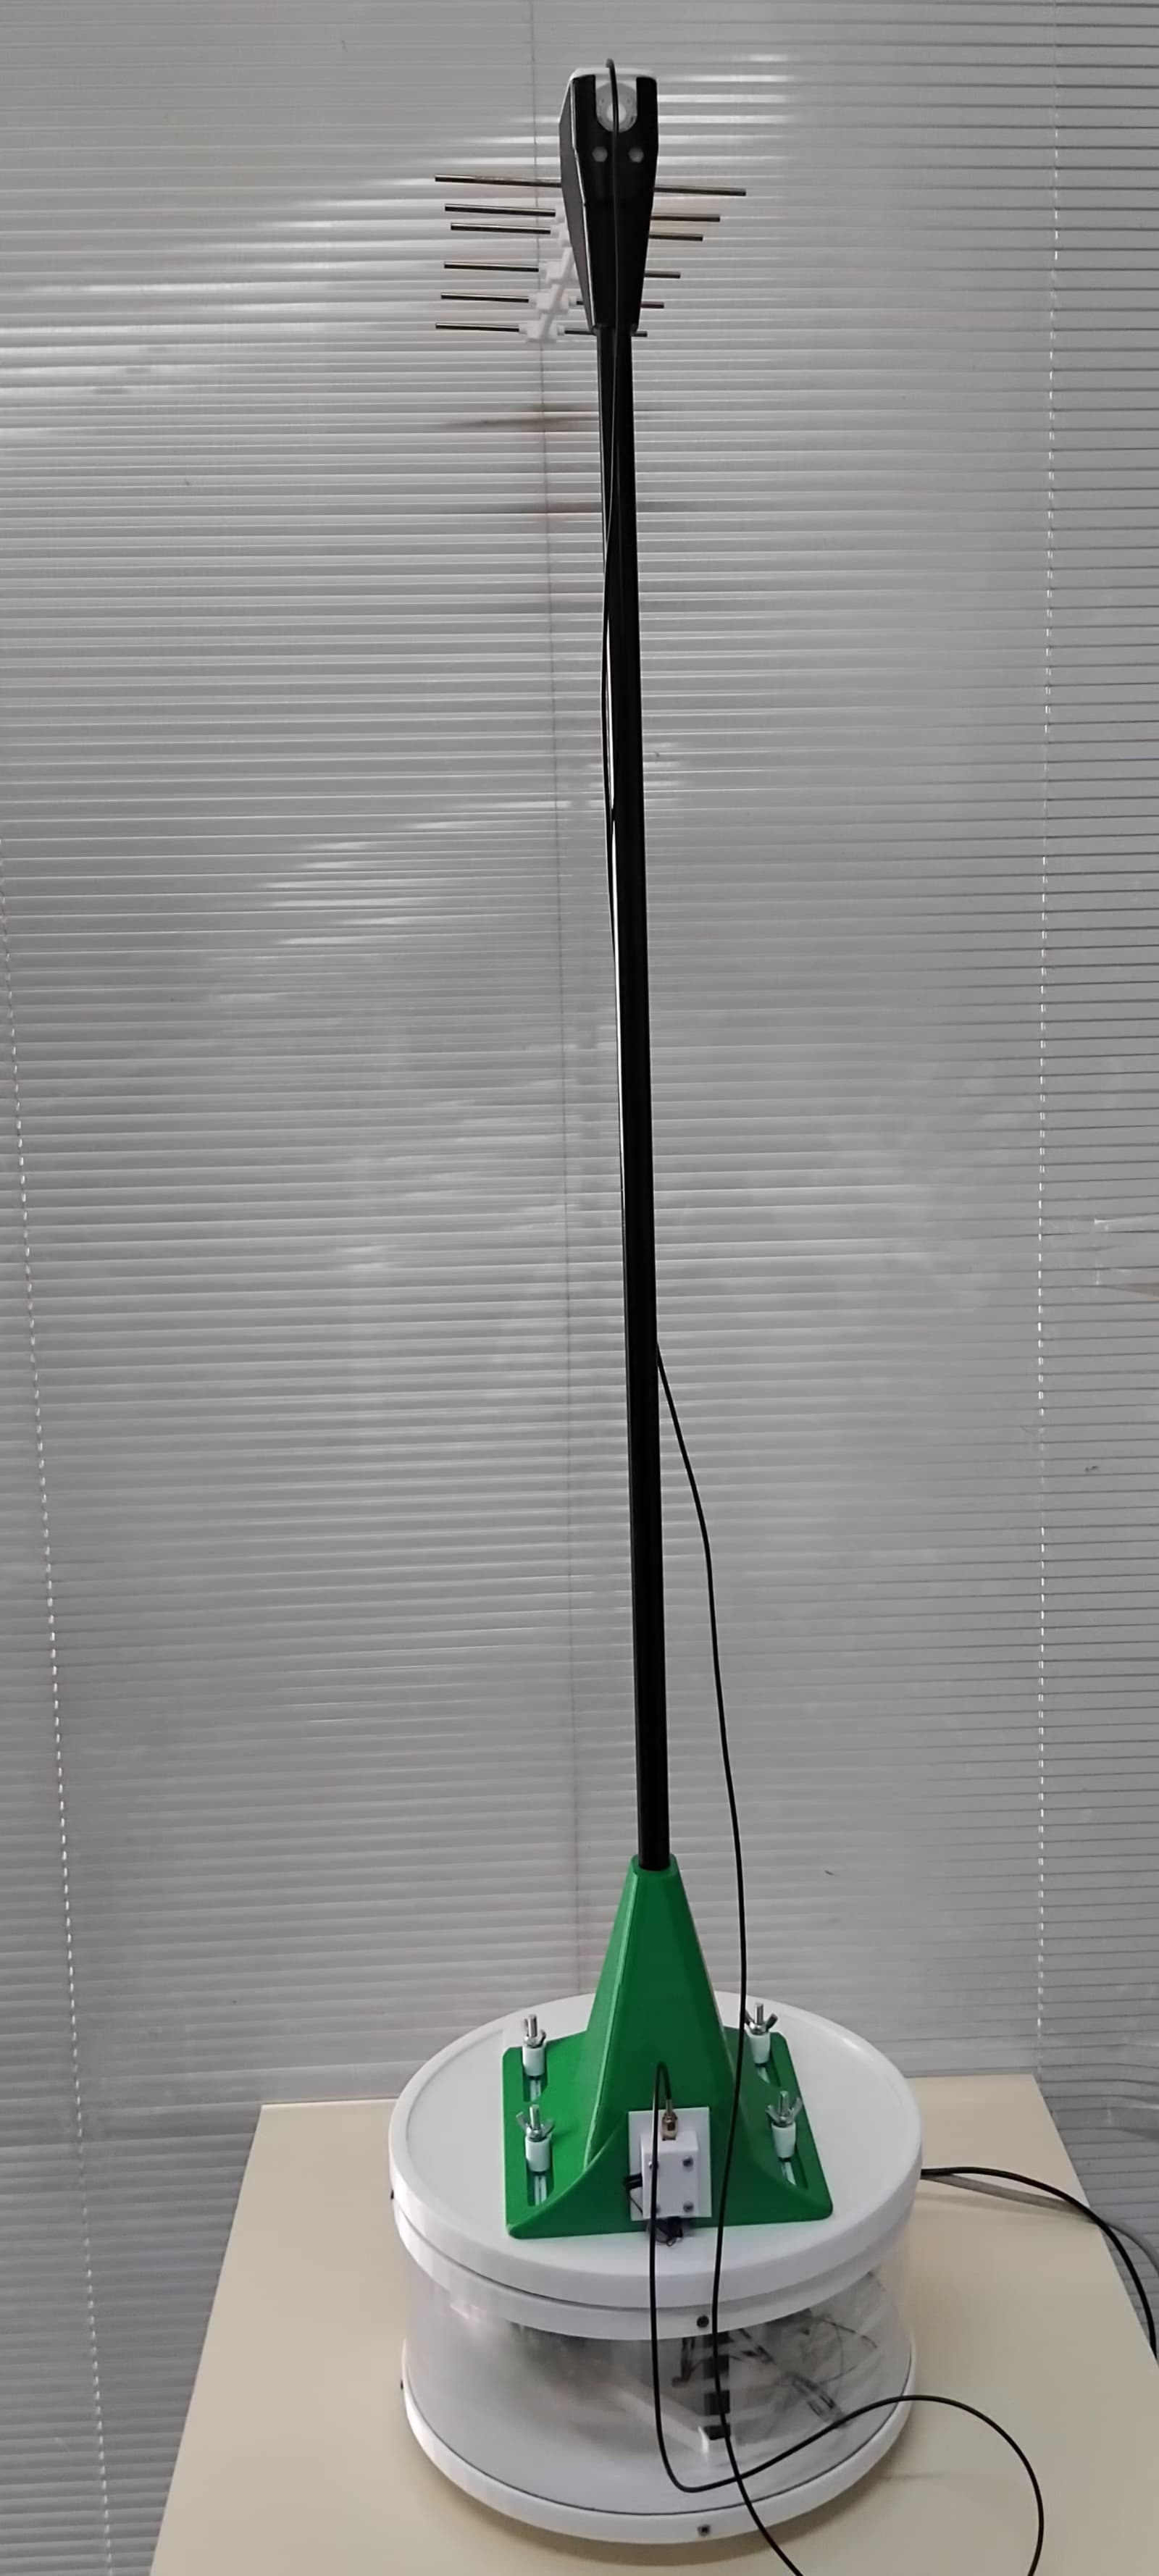
\includegraphics[width=\textwidth]{Imagens/back_view.jpg}
\caption{Back view}
\label{cap1:sec1:fig1:c}
\end{subfigure}
\caption{Overview of the complete antenna radiation pattern measurement system.}
\label{cap1:sec1:fig1}
\end{figure}

%-----------------------------------------------------------------------------------------------------
\section{Objectives}
%-----------------------------------------------------------------------------------------------------

The main objective of this work is to design and implement a low-cost computerised system for measuring antenna radiation patterns, suitable for educational and experimental use. This primary goal emphasises the development of a system that is accessible, reliable, and capable of providing meaningful practical experience in an academic context.

In addition to this, the project also addresses secondary objectives that contribute to the overall functionality and validation of the system. These include the construction of two Yagi–Uda antennas, to transmit and receive signals, the development of a two-axis rotating platform with angular control for antenna positioning, the integration of electronic subsystems for motor control, RF power detection, and data acquisition. Collectively, these secondary objectives support the achievement of the primary goal while ensuring the usability of the system and its educational usefulness.


%-----------------------------------------------------------------------------------------------------
\section{Document Structure}
%-----------------------------------------------------------------------------------------------------

The document is organised into five main chapters, each addressing a specific aspect of the work:

\begin{itemize}
    \item \textbf{Chapter 2 – State of the Art:} Reviews existing commercial antenna measurement systems and related research initiatives, emphasising the need for accessible, low-cost alternatives and setting the context for the proposed system.
    \item \textbf{Chapter 3 – Materials and Methods:} Describes the proposed system in detail, including its mechanical design, electronic subsystems, software development, and validation strategy. The chapter also covers the design and characterisation of the Yagi–Uda antenna, as well as the implementation of impedance matching and balun circuits.
    \item \textbf{Chapter 4 – Results:} Presents the experimental outcomes obtained from the characterisation of individual system components and the complete measurement setup, and compares them with simulated data to evaluate accuracy and repeatability.
    \item \textbf{Chapter 5 – Conclusions and Future Work:} Summarises the main findings, discusses limitations, and suggests ideas for future improvements.
\end{itemize}



%-----------------------------------------------------------------------------------------------------
\section{Scientific Publications}
%-----------------------------------------------------------------------------------------------------

The work developed in this project has also contributed to scientific publication. Two articles have already been produced: one presented at the \textit{5th Symposium of Applied Science for Young Researchers (SASYR)}, and another accepted for presentation at the \textit{13th Technological Ecosystems for Enhancing Multiculturality (TEEM)} conference, the latter being an indexed venue, which reinforces the scientific relevance of the results. 

In addition, the outcomes obtained from the design and validation of the Yagi–Uda antenna provide material for a potential third article, which may be developed in future work.
 